\documentclass[12pt,a4paper]{article}
\usepackage[utf8]{inputenc}
\usepackage[english]{babel}
\usepackage{geometry}
\usepackage{fancyhdr}
\usepackage{graphicx}
\usepackage{longtable}
\usepackage{array}
\usepackage{booktabs}
\usepackage{xcolor}
\usepackage{hyperref}
\usepackage{listings}
\usepackage{enumitem}
\usepackage{float}

\geometry{margin=1in}
\pagestyle{fancy}
\fancyhf{}
\rhead{\thepage}
\lhead{HIV Clinic RDS}

\title{\textbf{Requirements \& Design Specification\\HIV Clinic Management System}}
\author{Version: 2.0}
\date{January 2025}

\begin{document}

\maketitle
\thispagestyle{empty}

\newpage

\section*{Record of Changes}

\begin{longtable}{|p{2cm}|p{2cm}|p{1cm}|p{3cm}|p{6cm}|}
\hline
\textbf{Version} & \textbf{Date} & \textbf{A*M, D} & \textbf{In charge} & \textbf{Change Description} \\
\hline
V2.0 & 08/01/2025 & A & Development Team & Complete regeneration based on current codebase implementation \\
\hline
V2.0 & 08/01/2025 & A & Development Team & Updated requirements to reflect Spring Boot 3.2.0 architecture \\
\hline
V2.0 & 08/01/2025 & A & Development Team & Enhanced use cases and functional requirements \\
\hline
\end{longtable}

\textit{*A - Added M - Modified D - Deleted}

\newpage

\tableofcontents

\newpage

\section{Overview}

\subsection{Project Introduction}

The HIV Clinic Management System is a comprehensive web-based application designed to streamline healthcare operations for HIV/AIDS treatment facilities. The system provides integrated management of patient care, appointment scheduling, treatment tracking, and administrative functions while ensuring patient privacy and regulatory compliance.

\subsection{System Objectives}

\begin{itemize}
    \item Provide secure, role-based access to patient information and clinic resources
    \item Automate appointment scheduling and doctor availability management
    \item Track ARV (Antiretroviral) treatments and medication routines comprehensively
    \item Implement a robust notification system for appointment reminders and medication alerts
    \item Ensure patient data privacy with configurable privacy controls
    \item Support multi-role workflows for efficient clinic operations
    \item Maintain comprehensive audit trails for regulatory compliance
\end{itemize}

\subsection{Scope}

The system encompasses:
\begin{itemize}
    \item \textbf{User Management}: Multi-role authentication and authorization system
    \item \textbf{Patient Management}: Comprehensive patient profiles with privacy controls
    \item \textbf{Appointment System}: Advanced scheduling with conflict resolution
    \item \textbf{Medical Records}: Secure electronic health records management
    \item \textbf{Treatment Tracking}: ARV treatment plans and medication adherence monitoring
    \item \textbf{Notification System}: Template-based messaging and alert system
    \item \textbf{Administrative Functions}: User management, reporting, and system monitoring
\end{itemize}

\subsection{User Requirements}

\subsubsection{Actors}

The HIV Clinic Management System involves five primary actors with distinct roles and responsibilities:

\begin{longtable}{|p{1cm}|p{3cm}|p{10cm}|}
\hline
\textbf{\#} & \textbf{Actor} & \textbf{Description} \\
\hline
1 & Guest & Unregistered users who can view public information and register for patient accounts \\
\hline
2 & Patient & Registered HIV patients who manage appointments, view medical records, track treatments, and receive notifications \\
\hline
3 & Doctor & Healthcare providers who manage patient appointments, maintain medical records, prescribe treatments, and monitor patient progress \\
\hline
4 & Manager & Healthcare facility managers who oversee operations, generate reports, manage resources, and supervise clinic workflows \\
\hline
5 & Admin & System administrators with full access to user management, system configuration, and maintenance functions \\
\hline
\end{longtable}

\subsubsection{Use Cases}

\paragraph{a. Use Case Diagram}

\begin{figure}[H]
\centering
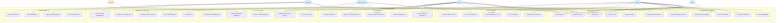
\includegraphics[width=0.9\textwidth]{diagrams/use_case_diagram}
\caption{HIV Clinic Management System Use Case Diagram}
\label{fig:use-case-diagram}
\end{figure}

The use case diagram illustrates the comprehensive interactions between system actors and the 35+ distinct use cases spanning authentication, appointment management, patient care, treatment tracking, and administrative functions.

\paragraph{b. Use Case Descriptions}

\begin{longtable}{|p{1cm}|p{3cm}|p{3cm}|p{7cm}|}
\hline
\textbf{ID} & \textbf{Use Case} & \textbf{Actor(s)} & \textbf{Description} \\
\hline
UC-001 & User Registration & Guest, Admin & New users register for patient accounts or admins create accounts for staff \\
\hline
UC-002 & User Authentication & All Users & Secure login using username/password with JWT token generation \\
\hline
UC-003 & Profile Management & All Users & Users can view and update their personal profile information \\
\hline
UC-004 & Change Password & All Users & Secure password change with validation and history tracking \\
\hline
UC-005 & Password Reset & All Users & Forgotten password reset via email verification \\
\hline
UC-006 & Book Appointment & Patient & Patients schedule appointments with available doctors \\
\hline
UC-007 & View Appointments & Patient, Doctor & Users view their scheduled appointments with details \\
\hline
UC-008 & Manage Availability & Doctor & Doctors set and modify their available time slots \\
\hline
UC-009 & Cancel Appointment & Patient, Doctor & Cancel appointments with automated notifications \\
\hline
UC-010 & Update Appointment Status & Doctor & Doctors update appointment status (completed, no-show, etc.) \\
\hline
UC-011 & View Medical Records & Patient, Doctor & Access patient medical history and records \\
\hline
UC-012 & Create Medical Record & Doctor & Doctors create new medical record entries \\
\hline
UC-013 & Update Medical Record & Doctor & Modify existing medical record information \\
\hline
UC-014 & Manage Privacy Settings & Patient & Patients control visibility of their medical information \\
\hline
UC-015 & Create Treatment Plan & Doctor & Doctors prescribe ARV treatment plans for patients \\
\hline
UC-016 & Monitor Treatment & Doctor, Patient & Track treatment progress and medication adherence \\
\hline
UC-017 & Manage Medication Routine & Patient, Doctor & Schedule and track daily medication routines \\
\hline
UC-018 & View Treatment History & Patient, Doctor & Access comprehensive treatment history \\
\hline
UC-019 & Send Notifications & System & Automated notifications for appointments and medications \\
\hline
UC-020 & View Notifications & All Users & Users view and manage their notifications \\
\hline
UC-021 & Manage Templates & Admin & Administrators manage notification templates \\
\hline
UC-022 & User Management & Admin, Manager & Create, modify, and deactivate user accounts \\
\hline
UC-023 & Generate Reports & Manager, Admin & Generate various clinic and patient reports \\
\hline
UC-024 & System Monitoring & Admin & Monitor system health and performance \\
\hline
UC-025 & Backup Data & Admin & Perform system and data backups \\
\hline
\end{longtable}

\section{Functional Requirements}

\subsection{Authentication and Authorization}

\subsubsection{FR-001: User Registration}
\begin{itemize}
    \item \textbf{Description}: System shall allow new users to register for patient accounts
    \item \textbf{Priority}: High
    \item \textbf{Requirements}:
    \begin{itemize}
        \item Unique username and email validation
        \item Secure password requirements (minimum 8 characters, mixed case, numbers)
        \item Email verification for account activation
        \item Role assignment (default: PATIENT)
        \item Account status tracking (active/inactive)
    \end{itemize}
\end{itemize}

\subsubsection{FR-002: User Authentication}
\begin{itemize}
    \item \textbf{Description}: System shall provide secure user authentication
    \item \textbf{Priority}: High
    \item \textbf{Requirements}:
    \begin{itemize}
        \item JWT-based stateless authentication
        \item Session timeout configuration (24 hours default)
        \item Concurrent session management
        \item Login activity tracking with IP and user agent
        \item Failed login attempt protection
    \end{itemize}
\end{itemize}

\subsubsection{FR-003: Role-Based Authorization}
\begin{itemize}
    \item \textbf{Description}: System shall enforce role-based access control
    \item \textbf{Priority}: High
    \item \textbf{Requirements}:
    \begin{itemize}
        \item Five distinct roles: Guest, Patient, Doctor, Manager, Admin
        \item Hierarchical permission structure
        \item Resource-based access control
        \item Method-level security enforcement
        \item Dynamic permission checking
    \end{itemize}
\end{itemize}

\subsection{Appointment Management}

\subsubsection{FR-004: Appointment Booking}
\begin{itemize}
    \item \textbf{Description}: Patients shall be able to book appointments with available doctors
    \item \textbf{Priority}: High
    \item \textbf{Requirements}:
    \begin{itemize}
        \item View doctor availability in real-time
        \item Select appointment time from available slots
        \item Automatic conflict detection and prevention
        \item Appointment confirmation with notification
        \item Support for recurring appointments
    \end{itemize}
\end{itemize}

\subsubsection{FR-005: Doctor Availability Management}
\begin{itemize}
    \item \textbf{Description}: Doctors shall manage their availability schedules
    \item \textbf{Priority}: High
    \item \textbf{Requirements}:
    \begin{itemize}
        \item Create, modify, and delete availability slots
        \item Set slot duration (default 30 minutes, configurable)
        \item Block time for non-patient activities
        \item Bulk availability management
        \item Holiday and leave management
    \end{itemize}
\end{itemize}

\subsubsection{FR-006: Appointment Status Management}
\begin{itemize}
    \item \textbf{Description}: System shall track appointment status lifecycle
    \item \textbf{Priority}: Medium
    \item \textbf{Requirements}:
    \begin{itemize}
        \item Status tracking: Scheduled, Confirmed, In Progress, Completed, Cancelled, No Show
        \item Status history with timestamps
        \item Automated status updates based on time
        \item Notification triggers for status changes
        \item Rescheduling capabilities
    \end{itemize}
\end{itemize}

\subsection{Patient Record Management}

\subsubsection{FR-007: Medical Record Creation}
\begin{itemize}
    \item \textbf{Description}: Doctors shall create comprehensive medical records
    \item \textbf{Priority}: High
    \item \textbf{Requirements}:
    \begin{itemize}
        \item Complete patient medical history capture
        \item Allergy and medication tracking
        \item Vital signs and examination notes
        \item Emergency contact information
        \item Structured data entry with validation
    \end{itemize}
\end{itemize}

\subsubsection{FR-008: Medical Record Access Control}
\begin{itemize}
    \item \textbf{Description}: System shall enforce privacy controls for medical records
    \item \textbf{Priority}: High
    \item \textbf{Requirements}:
    \begin{itemize}
        \item Patient-controlled privacy settings
        \item Role-based record access
        \item Data anonymization for private patients
        \item Audit trail for all record access
        \item Consent management for data sharing
    \end{itemize}
\end{itemize}

\subsubsection{FR-009: Medical Record History}
\begin{itemize}
    \item \textbf{Description}: System shall maintain complete medical record history
    \item \textbf{Priority}: Medium
    \item \textbf{Requirements}:
    \begin{itemize}
        \item Version control for record changes
        \item Change history with user attribution
        \item Record linking to appointments
        \item Historical data preservation
        \item Export capabilities for continuity of care
    \end{itemize}
\end{itemize}

\subsection{ARV Treatment Management}

\subsubsection{FR-010: Treatment Plan Creation}
\begin{itemize}
    \item \textbf{Description}: Doctors shall create and manage ARV treatment plans
    \item \textbf{Priority}: High
    \item \textbf{Requirements}:
    \begin{itemize}
        \item Medication selection from approved ARV list
        \item Dosage and frequency specification
        \item Treatment duration with start/end dates
        \item Side effect monitoring and documentation
        \item Drug interaction checking
    \end{itemize}
\end{itemize}

\subsubsection{FR-011: Medication Routine Management}
\begin{itemize}
    \item \textbf{Description}: System shall manage daily medication routines
    \item \textbf{Priority}: High
    \item \textbf{Requirements}:
    \begin{itemize}
        \item Daily medication scheduling
        \item Adherence tracking and reporting
        \item Reminder notifications
        \item Missed dose alerts
        \item Routine adjustment capabilities
    \end{itemize}
\end{itemize}

\subsubsection{FR-012: Treatment Monitoring}
\begin{itemize}
    \item \textbf{Description}: System shall support comprehensive treatment monitoring
    \item \textbf{Priority}: Medium
    \item \textbf{Requirements}:
    \begin{itemize}
        \item Treatment effectiveness tracking
        \item Side effect reporting
        \item Laboratory result integration
        \item Progress visualization and reporting
        \item Treatment plan adjustments
    \end{itemize}
\end{itemize}

\subsection{Notification System}

\subsubsection{FR-013: Automated Notifications}
\begin{itemize}
    \item \textbf{Description}: System shall send automated notifications
    \item \textbf{Priority}: Medium
    \item \textbf{Requirements}:
    \begin{itemize}
        \item Appointment reminders (configurable timing)
        \item Medication reminders based on routine
        \item Treatment milestone notifications
        \item System alerts and announcements
        \item Escalation for missed appointments
    \end{itemize}
\end{itemize}

\subsubsection{FR-014: Notification Templates}
\begin{itemize}
    \item \textbf{Description}: System shall support template-based messaging
    \item \textbf{Priority}: Low
    \item \textbf{Requirements}:
    \begin{itemize}
        \item Configurable message templates
        \item Variable substitution in templates
        \item Multi-language template support
        \item Template versioning and management
        \item A/B testing for message effectiveness
    \end{itemize}
\end{itemize}

\subsubsection{FR-015: Notification Delivery}
\begin{itemize}
    \item \textbf{Description}: System shall deliver notifications through multiple channels
    \item \textbf{Priority}: Medium
    \item \textbf{Requirements}:
    \begin{itemize}
        \item In-app notification center
        \item Email notification delivery
        \item SMS integration capability
        \item Push notification support
        \item Delivery status tracking
    \end{itemize}
\end{itemize}

\subsection{Administrative Functions}

\subsubsection{FR-016: User Management}
\begin{itemize}
    \item \textbf{Description}: Administrators shall manage system users
    \item \textbf{Priority}: High
    \item \textbf{Requirements}:
    \begin{itemize}
        \item Create accounts for staff members
        \item Modify user roles and permissions
        \item Activate/deactivate user accounts
        \item Password reset capabilities
        \item User activity monitoring
    \end{itemize}
\end{itemize}

\subsubsection{FR-017: System Monitoring}
\begin{itemize}
    \item \textbf{Description}: System shall provide monitoring and health check capabilities
    \item \textbf{Priority}: Medium
    \item \textbf{Requirements}:
    \begin{itemize}
        \item Application health monitoring
        \item Database performance tracking
        \item User session monitoring
        \item Error logging and alerting
        \item Performance metrics collection
    \end{itemize}
\end{itemize}

\subsubsection{FR-018: Reporting and Analytics}
\begin{itemize}
    \item \textbf{Description}: System shall generate comprehensive reports
    \item \textbf{Priority}: Medium
    \item \textbf{Requirements}:
    \begin{itemize}
        \item Patient statistics and demographics
        \item Appointment analytics and trends
        \item Treatment effectiveness reports
        \item System usage analytics
        \item Export capabilities (PDF, Excel)
    \end{itemize}
\end{itemize}

\section{Non-Functional Requirements}

\subsection{Performance Requirements}

\subsubsection{NFR-001: Response Time}
\begin{itemize}
    \item \textbf{Requirement}: System response time shall not exceed 3 seconds for 95\% of requests
    \item \textbf{Measurement}: Average response time under normal load
    \item \textbf{Implementation}: Database indexing, connection pooling, query optimization
\end{itemize}

\subsubsection{NFR-002: Throughput}
\begin{itemize}
    \item \textbf{Requirement}: System shall support minimum 100 concurrent users
    \item \textbf{Measurement}: Load testing with simulated users
    \item \textbf{Implementation}: Stateless architecture, horizontal scaling capability
\end{itemize}

\subsubsection{NFR-003: Scalability}
\begin{itemize}
    \item \textbf{Requirement}: System shall scale to 1000+ users with minimal performance degradation
    \item \textbf{Measurement}: Performance under increased load
    \item \textbf{Implementation}: Microservice-ready architecture, database partitioning
\end{itemize}

\subsection{Security Requirements}

\subsubsection{NFR-004: Data Encryption}
\begin{itemize}
    \item \textbf{Requirement}: All sensitive data shall be encrypted in transit and at rest
    \item \textbf{Implementation}: HTTPS/TLS for transmission, database encryption for storage
    \item \textbf{Compliance}: HIPAA compliance for healthcare data protection
\end{itemize}

\subsubsection{NFR-005: Authentication Security}
\begin{itemize}
    \item \textbf{Requirement}: Strong authentication with secure password policies
    \item \textbf{Implementation}: BCrypt password hashing, JWT tokens, session management
    \item \textbf{Features}: Account lockout, password complexity requirements
\end{itemize}

\subsubsection{NFR-006: Access Control}
\begin{itemize}
    \item \textbf{Requirement}: Strict role-based access control with audit trails
    \item \textbf{Implementation}: Spring Security, method-level authorization
    \item \textbf{Features}: Resource-based permissions, activity logging
\end{itemize}

\subsection{Reliability Requirements}

\subsubsection{NFR-007: System Availability}
\begin{itemize}
    \item \textbf{Requirement}: System uptime of 99.5\% during business hours
    \item \textbf{Measurement}: Monitoring and alerting systems
    \item \textbf{Implementation}: Robust error handling, graceful degradation
\end{itemize}

\subsubsection{NFR-008: Data Integrity}
\begin{itemize}
    \item \textbf{Requirement}: Zero data loss with automatic backup and recovery
    \item \textbf{Implementation}: Database transactions, regular backups
    \item \textbf{Features}: Point-in-time recovery, data validation
\end{itemize}

\subsubsection{NFR-009: Fault Tolerance}
\begin{itemize}
    \item \textbf{Requirement}: System shall continue operating with component failures
    \item \textbf{Implementation}: Circuit breakers, retry mechanisms
    \item \textbf{Features}: Health checks, automatic failover
\end{itemize}

\subsection{Usability Requirements}

\subsubsection{NFR-010: User Interface}
\begin{itemize}
    \item \textbf{Requirement}: Intuitive, responsive web interface
    \item \textbf{Implementation}: React-based SPA with modern UI components
    \item \textbf{Features}: Mobile-responsive design, accessibility compliance
\end{itemize}

\subsubsection{NFR-011: User Experience}
\begin{itemize}
    \item \textbf{Requirement}: Consistent navigation and workflow across all user roles
    \item \textbf{Implementation}: Role-based UI customization, context-aware menus
    \item \textbf{Features}: Progressive disclosure, task-oriented design
\end{itemize}

\subsubsection{NFR-012: Documentation}
\begin{itemize}
    \item \textbf{Requirement}: Comprehensive user documentation and help system
    \item \textbf{Implementation}: Inline help, user guides, video tutorials
    \item \textbf{Features}: Context-sensitive help, searchable knowledge base
\end{itemize}

\section{System Architecture}

\subsection{Architecture Overview}

\begin{figure}[H]
\centering
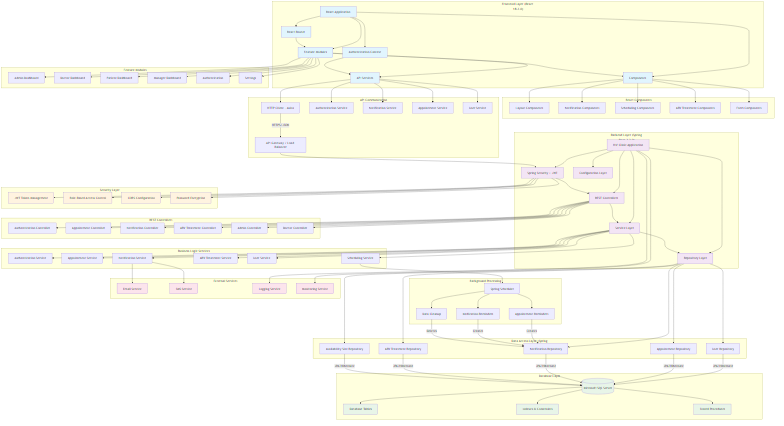
\includegraphics[width=0.9\textwidth]{diagrams/system_architecture}
\caption{System Architecture Diagram}
\label{fig:system-architecture}
\end{figure}

The HIV Clinic Management System implements a modern three-tier architecture:

\subsubsection{Presentation Layer}
\begin{itemize}
    \item \textbf{Technology}: React 18.2.0 with Vite build system
    \item \textbf{Features}: Single-page application with client-side routing
    \item \textbf{Components}: Role-based UI, responsive design, real-time updates
    \item \textbf{State Management}: Context API for global state, local state for components
\end{itemize}

\subsubsection{Business Logic Layer}
\begin{itemize}
    \item \textbf{Technology}: Spring Boot 3.2.0 with Java 17
    \item \textbf{Architecture}: RESTful web services with layered design
    \item \textbf{Security}: Spring Security with JWT authentication
    \item \textbf{Features}: Transaction management, validation, audit logging
\end{itemize}

\subsubsection{Data Layer}
\begin{itemize}
    \item \textbf{Technology}: Microsoft SQL Server with Hibernate JPA
    \item \textbf{Features}: ACID compliance, referential integrity, indexing
    \item \textbf{Performance}: Connection pooling, query optimization
    \item \textbf{Backup}: Automated backups with point-in-time recovery
\end{itemize}

\subsection{Component Interactions}

\begin{figure}[H]
\centering
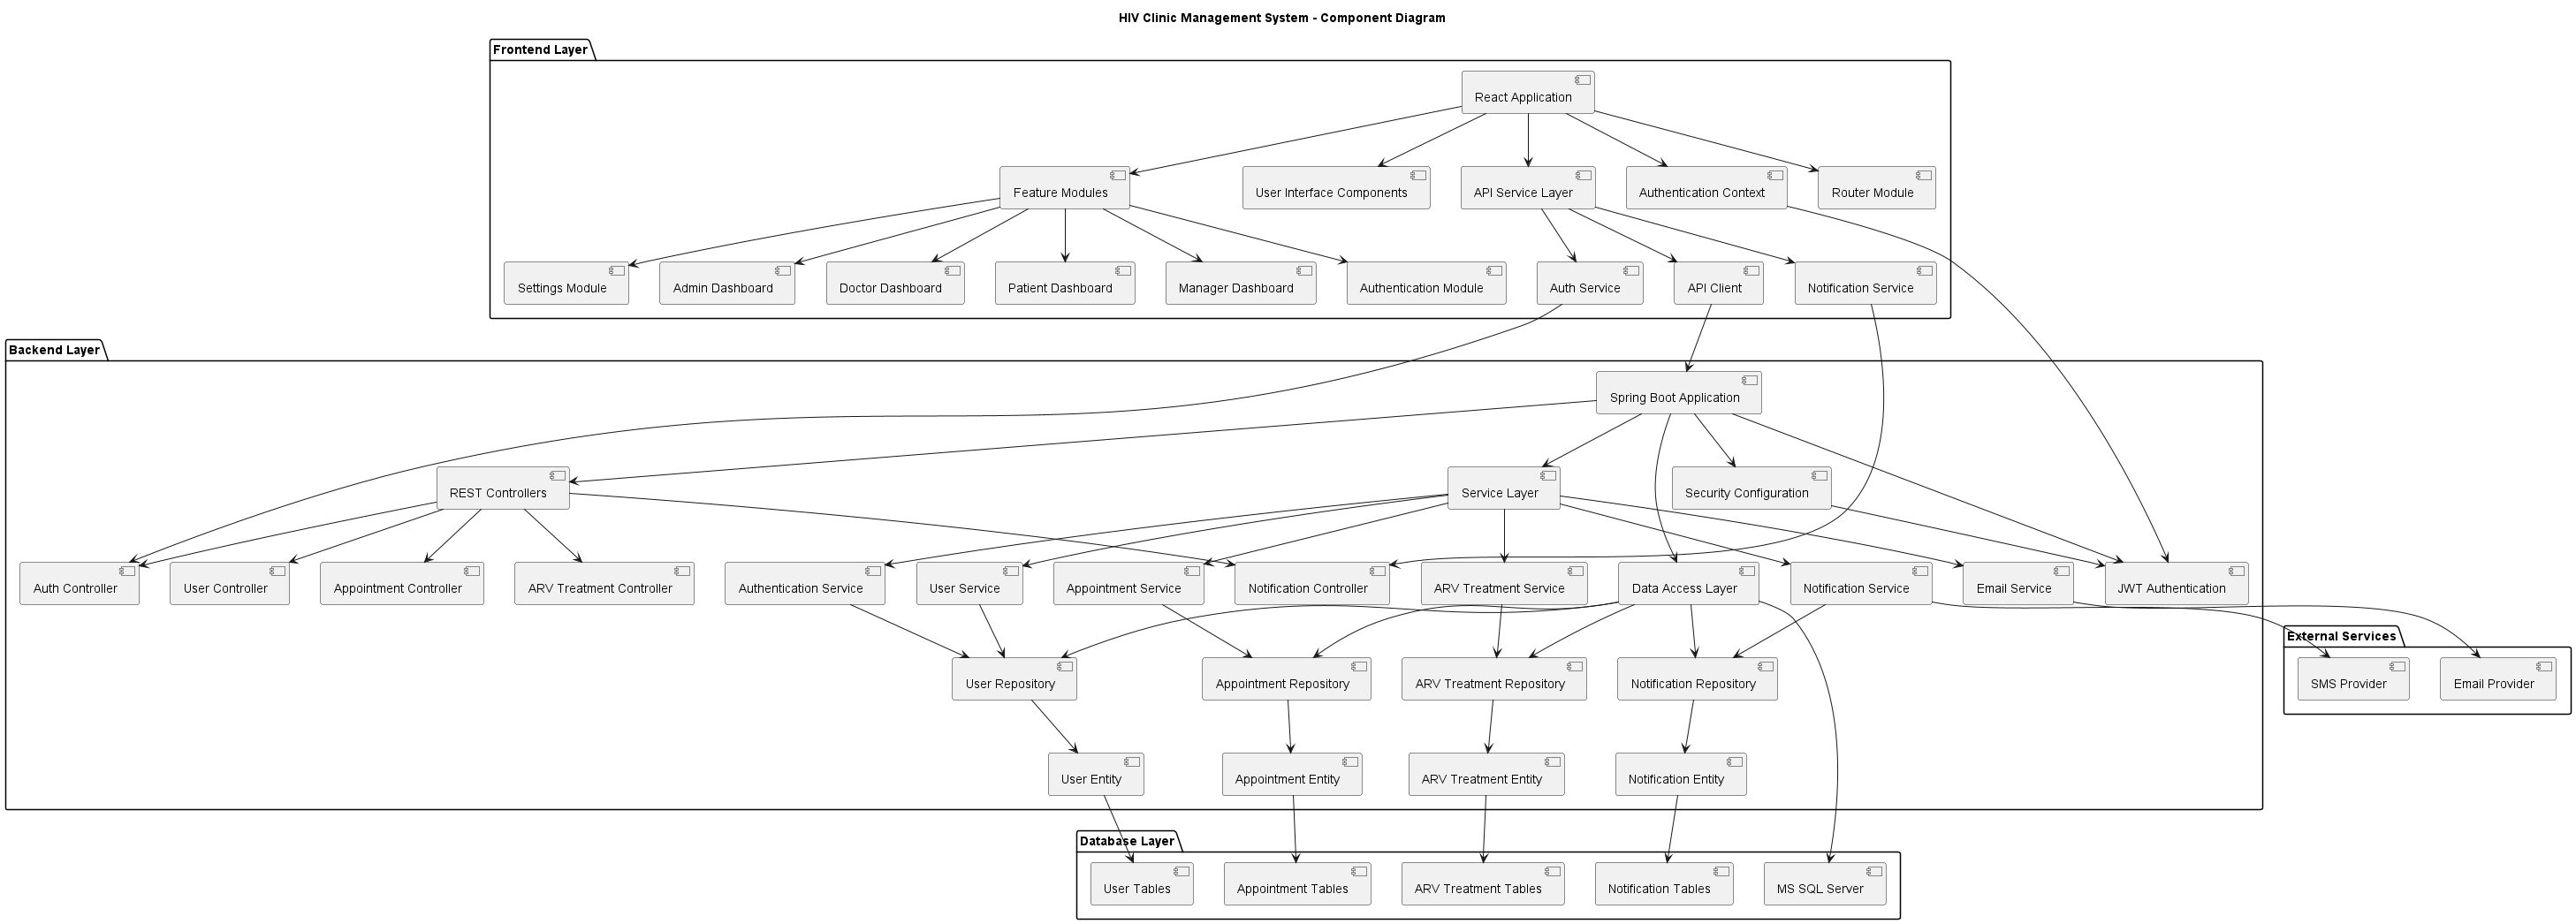
\includegraphics[width=0.9\textwidth]{diagrams/component_diagram}
\caption{Component Interaction Diagram}
\label{fig:component-diagram}
\end{figure}

\subsubsection{Authentication Flow}
\begin{figure}[H]
\centering
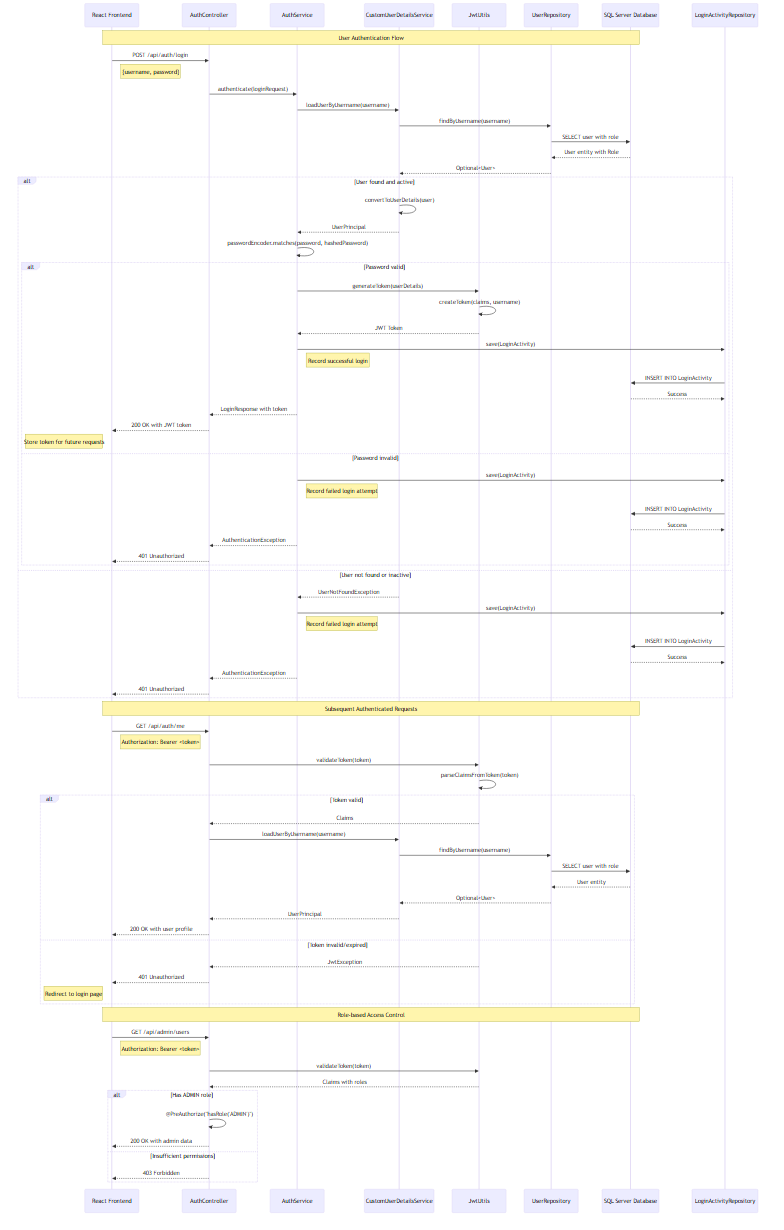
\includegraphics[width=0.9\textwidth]{diagrams/authentication_sequence}
\caption{Authentication Sequence Diagram}
\label{fig:authentication-sequence}
\end{figure}

The authentication process follows these steps:
\begin{enumerate}
    \item User submits credentials to AuthController
    \item AuthService validates credentials against User repository
    \item JWT token generated with user role and permissions
    \item Token returned to client for subsequent requests
    \item Client includes token in Authorization header
    \item Security filter validates token on each request
\end{enumerate}

\subsubsection{Appointment Booking Flow}
\begin{figure}[H]
\centering
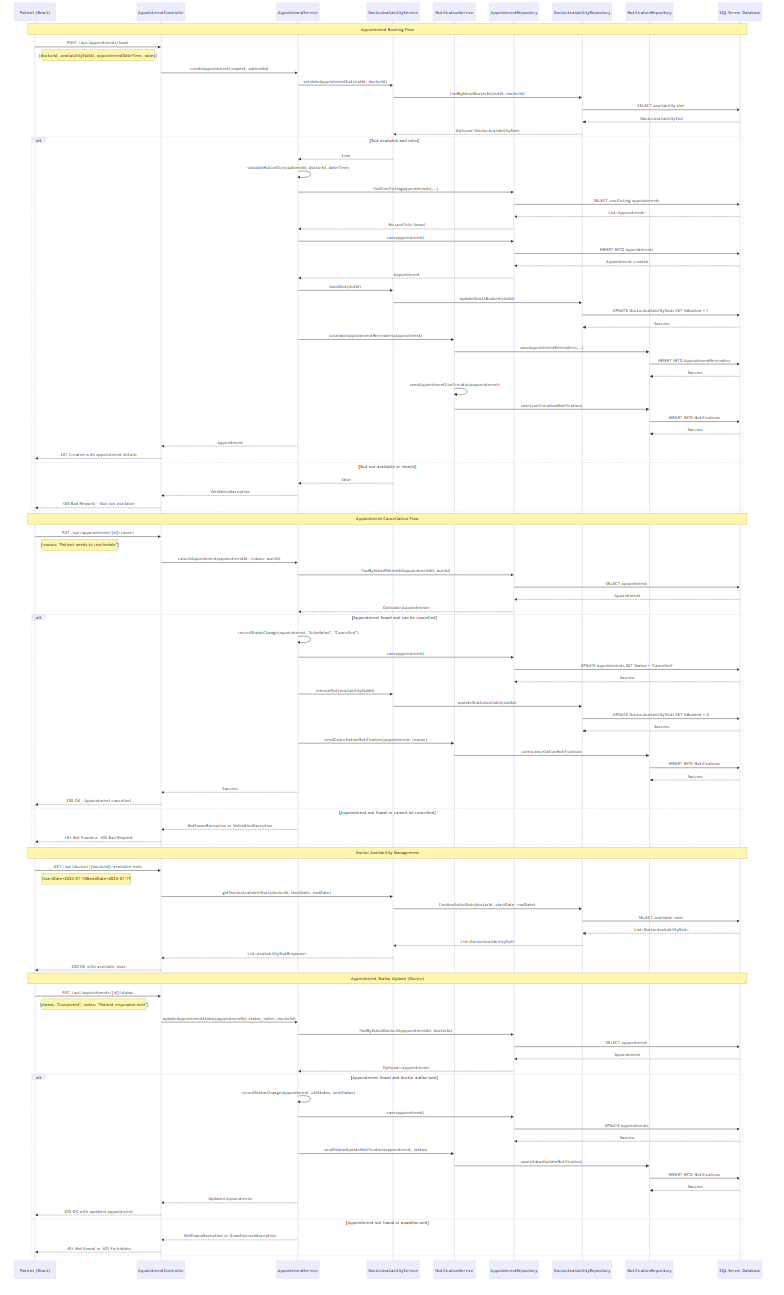
\includegraphics[width=0.9\textwidth]{diagrams/appointment_booking_sequence}
\caption{Appointment Booking Sequence Diagram}
\label{fig:appointment-sequence}
\end{figure}

The appointment booking process includes:
\begin{enumerate}
    \item Patient views available doctor slots
    \item System checks availability in real-time
    \item Patient selects preferred time slot
    \item System validates appointment constraints
    \item Appointment created with notification triggers
    \item Confirmation sent to both patient and doctor
\end{enumerate}

\subsection{Data Model}

\begin{figure}[H]
\centering
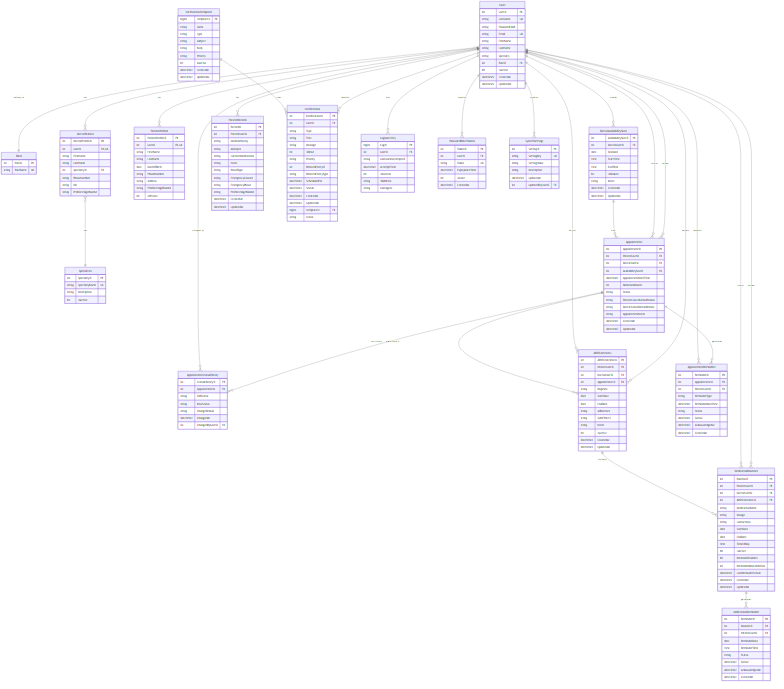
\includegraphics[width=0.9\textwidth]{diagrams/database_schema_erd}
\caption{Database Entity Relationship Diagram}
\label{fig:database-erd}
\end{figure}

\subsubsection{Core Entities}

\paragraph{User Management}
\begin{itemize}
    \item \textbf{Users}: Central user table with role-based access
    \item \textbf{Roles}: Role definitions for authorization
    \item \textbf{UserSessions}: Active session tracking
    \item \textbf{LoginActivity}: Authentication audit trail
\end{itemize}

\paragraph{Patient Management}
\begin{itemize}
    \item \textbf{PatientProfiles}: Extended patient information
    \item \textbf{PatientRecords}: Medical records with privacy controls
    \item \textbf{DoctorProfiles}: Healthcare provider information
\end{itemize}

\paragraph{Appointment System}
\begin{itemize}
    \item \textbf{Appointments}: Core appointment data
    \item \textbf{DoctorAvailabilitySlots}: Doctor schedule management
    \item \textbf{AppointmentStatusHistory}: Status change tracking
\end{itemize}

\paragraph{Treatment Management}
\begin{itemize}
    \item \textbf{ARVTreatments}: Antiretroviral treatment plans
    \item \textbf{MedicationRoutines}: Daily medication schedules
    \item \textbf{SystemSettings}: Configurable system parameters
\end{itemize}

\paragraph{Notification System}
\begin{itemize}
    \item \textbf{Notifications}: Message delivery tracking
    \item \textbf{NotificationTemplates}: Template-based messaging
\end{itemize}

\section{Technical Specifications}

\subsection{Technology Stack}

\subsubsection{Backend Technologies}
\begin{longtable}{|p{3cm}|p{2cm}|p{7cm}|}
\hline
\textbf{Component} & \textbf{Version} & \textbf{Purpose} \\
\hline
Java & 17 LTS & Core programming language with enhanced performance \\
\hline
Spring Boot & 3.2.0 & Application framework with embedded server \\
\hline
Spring Security & 6.x & Authentication and authorization \\
\hline
Spring Data JPA & 3.x & Data persistence with repository pattern \\
\hline
Hibernate & 6.x & Object-relational mapping \\
\hline
Microsoft SQL Server & 2019+ & Primary database management system \\
\hline
HikariCP & Latest & High-performance connection pooling \\
\hline
Maven & 3.8+ & Dependency management and build tool \\
\hline
Lombok & Latest & Code generation for reducing boilerplate \\
\hline
\end{longtable}

\subsubsection{Frontend Technologies}
\begin{longtable}{|p{3cm}|p{2cm}|p{7cm}|}
\hline
\textbf{Component} & \textbf{Version} & \textbf{Purpose} \\
\hline
React & 18.2.0 & UI library with concurrent features \\
\hline
React Router DOM & 6.8.0 & Client-side routing and navigation \\
\hline
Vite & 7.0.2 & Fast build tool and development server \\
\hline
Axios & 1.6.0 & HTTP client for API communication \\
\hline
Vitest & Latest & Unit testing framework \\
\hline
React Testing Library & Latest & Component testing utilities \\
\hline
ESLint & Latest & Code quality and style enforcement \\
\hline
\end{longtable}

\subsection{Development Environment}

\subsubsection{Development Setup}
\begin{itemize}
    \item \textbf{IDE}: IntelliJ IDEA or Visual Studio Code
    \item \textbf{Java SDK}: OpenJDK 17 or higher
    \item \textbf{Node.js}: Version 18+ for frontend development
    \item \textbf{Database}: SQL Server 2019 Developer Edition
    \item \textbf{Version Control}: Git with GitHub repository
\end{itemize}

\subsubsection{Build and Deployment}
\begin{itemize}
    \item \textbf{Backend Build}: Maven with Spring Boot plugin
    \item \textbf{Frontend Build}: Vite with production optimization
    \item \textbf{Containerization}: Docker with multi-stage builds
    \item \textbf{Orchestration}: Docker Compose for local development
\end{itemize}

\subsection{API Design Standards}

\subsubsection{RESTful Principles}
\begin{itemize}
    \item Resource-based URLs with consistent naming conventions
    \item HTTP methods for CRUD operations (GET, POST, PUT, DELETE)
    \item Stateless interactions with JWT token authentication
    \item JSON request/response format with standardized error handling
    \item HATEOAS links for related resources
\end{itemize}

\subsubsection{Response Format}
\begin{lstlisting}[language=JSON]
{
  "success": true,
  "message": "Operation completed successfully",
  "data": {
    // Response payload
  },
  "timestamp": "2025-01-08T10:30:00Z",
  "pagination": {
    "page": 1,
    "size": 20,
    "total": 100
  }
}
\end{lstlisting}

\subsubsection{Error Handling}
\begin{lstlisting}[language=JSON]
{
  "success": false,
  "error": {
    "code": "VALIDATION_ERROR",
    "message": "Invalid input data",
    "details": [
      {
        "field": "email",
        "message": "Email format is invalid"
      }
    ]
  },
  "timestamp": "2025-01-08T10:30:00Z"
}
\end{lstlisting}

\section{Security Design}

\subsection{Authentication Mechanism}

\subsubsection{JWT Token Structure}
JSON Web Tokens contain the following claims for secure authentication:

\begin{lstlisting}[language=JSON]
{
  "sub": "username",
  "userId": 123,
  "roleId": 2,
  "roleName": "DOCTOR",
  "iat": 1704715200,
  "exp": 1704801600,
  "jti": "token-id-12345"
}
\end{lstlisting}

\subsubsection{Password Security}
\begin{itemize}
    \item \textbf{Hashing}: BCrypt with configurable strength (default: 12)
    \item \textbf{Policy}: Minimum 8 characters, mixed case, numbers, special characters
    \item \textbf{History}: Previous 5 passwords stored to prevent reuse
    \item \textbf{Expiration}: Optional password expiration (disabled by default)
    \item \textbf{Reset}: Secure token-based password reset with time limits
\end{itemize}

\subsection{Authorization Matrix}

\begin{longtable}{|p{2.5cm}|p{1.5cm}|p{1.5cm}|p{1.5cm}|p{1.5cm}|p{1.5cm}|}
\hline
\textbf{Resource/Action} & \textbf{Guest} & \textbf{Patient} & \textbf{Doctor} & \textbf{Manager} & \textbf{Admin} \\
\hline
Register Account & ✓ & - & - & ✓ & ✓ \\
\hline
Login/Logout & ✓ & ✓ & ✓ & ✓ & ✓ \\
\hline
View Profile & - & ✓ & ✓ & ✓ & ✓ \\
\hline
Book Appointment & - & ✓ & - & - & ✓ \\
\hline
View Own Appointments & - & ✓ & ✓ & ✓ & ✓ \\
\hline
View All Appointments & - & - & ✓ & ✓ & ✓ \\
\hline
Manage Availability & - & - & ✓ & ✓ & ✓ \\
\hline
View Own Records & - & ✓ & - & - & ✓ \\
\hline
View Patient Records & - & - & ✓ & ✓ & ✓ \\
\hline
Create Records & - & - & ✓ & - & ✓ \\
\hline
Manage Treatments & - & ✓ & ✓ & ✓ & ✓ \\
\hline
User Management & - & - & - & ✓ & ✓ \\
\hline
System Settings & - & - & - & ✓ & ✓ \\
\hline
Generate Reports & - & - & - & ✓ & ✓ \\
\hline
\end{longtable}

\subsection{Data Protection}

\subsubsection{Patient Privacy Controls}
\begin{itemize}
    \item \textbf{Privacy Flag}: Boolean setting to enable/disable data anonymization
    \item \textbf{Data Masking}: Automatic masking of PII for private patients
    \item \textbf{Access Logging}: Complete audit trail of medical record access
    \item \textbf{Consent Management}: Patient consent tracking for data sharing
    \item \textbf{Data Retention}: Configurable retention policies for inactive records
\end{itemize}

\subsubsection{Encryption Standards}
\begin{itemize}
    \item \textbf{Transport}: TLS 1.3 for all client-server communication
    \item \textbf{Storage}: Database-level encryption for sensitive fields
    \item \textbf{Backup}: Encrypted backup files with separate key management
    \item \textbf{Configuration}: Secure configuration management for secrets
\end{itemize}

\section{Testing Strategy}

\subsection{Testing Pyramid}

\subsubsection{Unit Testing}
\begin{itemize}
    \item \textbf{Backend}: JUnit 5 with Mockito for service layer testing
    \item \textbf{Frontend}: Vitest for component and utility testing
    \item \textbf{Coverage}: Minimum 80\% code coverage requirement
    \item \textbf{Automation}: Continuous testing in CI/CD pipeline
\end{itemize}

\subsubsection{Integration Testing}
\begin{itemize}
    \item \textbf{API Testing}: Spring Boot Test for endpoint testing
    \item \textbf{Database Testing}: TestContainers for data layer testing
    \item \textbf{Security Testing}: Spring Security Test for authentication
    \item \textbf{Component Testing}: React Testing Library for UI components
\end{itemize}

\subsubsection{End-to-End Testing}
\begin{itemize}
    \item \textbf{User Workflows}: Complete user journey testing
    \item \textbf{Cross-Browser}: Testing across major browsers
    \item \textbf{Mobile Testing}: Responsive design validation
    \item \textbf{Performance Testing}: Load testing for scalability
\end{itemize}

\subsection{Quality Assurance}

\subsubsection{Code Quality}
\begin{itemize}
    \item \textbf{Static Analysis}: SonarQube for code quality metrics
    \item \textbf{Code Reviews}: Peer review process for all changes
    \item \textbf{Coding Standards}: Consistent style guide enforcement
    \item \textbf{Documentation}: Comprehensive code and API documentation
\end{itemize}

\subsubsection{Security Testing}
\begin{itemize}
    \item \textbf{Vulnerability Scanning}: Automated security scans
    \item \textbf{Penetration Testing}: Regular security assessments
    \item \textbf{Dependency Checking}: Automated dependency vulnerability scanning
    \item \textbf{Compliance Validation}: HIPAA compliance verification
\end{itemize}

\section{Deployment and Operations}

\subsection{Deployment Architecture}

\subsubsection{Production Environment}
\begin{itemize}
    \item \textbf{Application Server}: Load-balanced Spring Boot instances
    \item \textbf{Web Server}: Nginx reverse proxy with SSL termination
    \item \textbf{Database}: SQL Server cluster with high availability
    \item \textbf{Monitoring}: Application and infrastructure monitoring
\end{itemize}

\subsubsection{Scalability Considerations}
\begin{itemize}
    \item \textbf{Horizontal Scaling}: Stateless application design
    \item \textbf{Database Optimization}: Indexing and query optimization
    \item \textbf{Caching Strategy}: Redis for session and data caching
    \item \textbf{CDN Integration}: Content delivery for static assets
\end{itemize}

\subsection{Monitoring and Maintenance}

\subsubsection{Application Monitoring}
\begin{itemize}
    \item \textbf{Health Checks}: Automated health monitoring endpoints
    \item \textbf{Performance Metrics}: Response time and throughput tracking
    \item \textbf{Error Logging}: Centralized logging with alerting
    \item \textbf{User Analytics}: Usage patterns and system adoption
\end{itemize}

\subsubsection{Backup and Recovery}
\begin{itemize}
    \item \textbf{Database Backups}: Daily full backups with transaction log backups
    \item \textbf{Application Backups}: Configuration and deployment artifacts
    \item \textbf{Recovery Testing}: Regular recovery procedure validation
    \item \textbf{Disaster Recovery}: Geographic redundancy for critical data
\end{itemize}

\section{Conclusion}

The HIV Clinic Management System Requirements and Design Specification provides a comprehensive foundation for developing a robust, secure, and user-friendly healthcare management platform. The system addresses the unique needs of HIV treatment facilities while ensuring compliance with healthcare regulations and best practices.

The modular architecture and modern technology stack position the system for future enhancements and scalability. The emphasis on security, privacy, and audit trails ensures the protection of sensitive patient information while enabling efficient clinical workflows.

Implementation of this specification will result in a system that significantly improves clinic operations, enhances patient care, and provides valuable insights for healthcare providers and administrators.

\end{document}